%Tex root = Linguaggi.tex

\chapter{Espressioni}
Le \textcolor{colore}{\textbf{espressioni}} sono la categoria sintattica il cui significato è un valore ottenuto mediante una valutazione.

\section{Dscrivere le espressioni}
Il valore ottenuto mediante la valutazione di un'espressione è detto \textcolor{colore}{\textbf{valore esprimibile}}, in quanto è un valore che può essere espresso attraverso la sintassi dei linguaggi di programmazione (sintassi delle espressioni).

\begin{mydef}{valore esprimibile}
    Un \textbf{valore esprimibile} è definito come:
    \begin{equation*}
        \mathrm{Eval} = \underbrace{\mathrm{int}}_{\mathbb{Z}} \cup \underbrace{\mathrm{bool}}_{\mathrm{\{true, \ false\}}}
    \end{equation*}
\end{mydef}

Gli aspetti che caratterizzano le espressioni sono:
\begin{itemize}[label=$\triangleright$, itemsep=\smallskipamount]
    \item \textbf{arietà degli operatori} e \textbf{notazione}:
    \item \textbf{regole di precedenza} (tra operatori)
    \item \textbf{regole di associa} (degli operatori)
    \item \textbf{ordine di valutazione degli operandi}
    \item \textbf{presenza di side effect}
    \item \textbf{overloading degli operatori}
    \item \textbf{espressioni con tipi misti}
\end{itemize}

\subsection{Notazione}
Le espressioni possono essere denotate in modo diversi:
\begin{itemize}[label=$\circ$, itemsep=\smallskipamount]
    \item \textbf{notazione in-fissa}: \texttt{a + b}
    \item \textbf{notazione pre-fissa}: \texttt{+ a b}
    \item \textbf{notazione post-fissa}: \texttt{a b +}
\end{itemize}

La scelta della notazione può determinare le regole di associatività e/o precedenza, o incidere su altre caratteristiche delle espressioni.

\subsubsection{Notazione in-fissa}
La \textcolor{colore}{\textbf{notazione in-fissa}} è quella più usata in matematica.\\[0.2ex]
Questa notazione, infatti, è quella che permette una lettura più intuitiva, ma richiede maggiori specifiche.\\[0.2ex]
Per prima cosa, però, è necessario stabilire le regole di precedenza e associatività.\\[0.2ex]
Inoltre, è necessario l'utilizzo delle parentesi per permettere precedenze o associatività diverse da quelle regole o aumentare la leggibilità.

\begin{figure}[H]
    \centering
    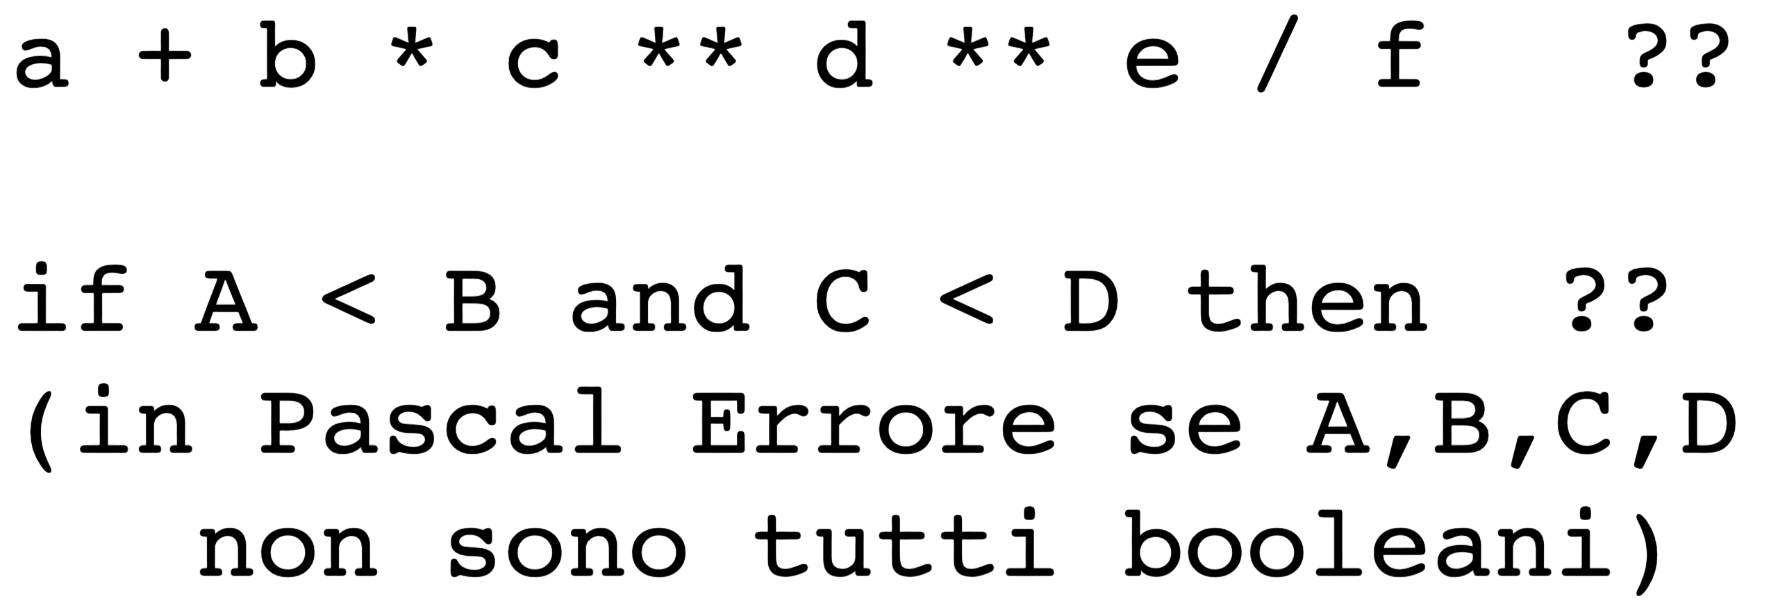
\includegraphics[width=0.5\textwidth]{images/notazione-inFissa.png}
\end{figure}

\subsubsection{Notazione pre-fissa}
La \textcolor{colore}{\textbf{notazione pre-fissa}} è più semplice dell'in-fissa in quanto non necessita di regole di precedenza e associatività, e non necessita nemmeno di parentesi.

\vario{Algoritmo di valutazione}{
    \centering
    \begin{minipage}[c]{0.5\textwidth}
        \begin{enumerate}[itemsep=\smallskipamount]
            \item leggere il prossimo simbolo dell’espressione e metterlo nella pila
            \item se il simbolo è un operatore \texttt{op}:\texttt{ Cop = n} e torna a 1
            \item se il simbolo letto è un operando inserirlo nella pila e calcola \texttt{Cop = Cop - 1} (\texttt{op} ultimo operatore inserito)
            \item se \texttt{Cop != 0} torna a 1 (op ultimo operatore inserito)
            \item se \texttt{Cop = 0} allora:
            \begin{itemize}[itemsep=\smallskipamount]
                \item applicare l’ultimo operatore op agli operandi in cima alla pila (che vanno cancellati) e caricare il risultato nella pila e se non ci sono più simboli vai a 6
                \item  \texttt{Cop = n - m} (\texttt{n} arietà del nuovo ultimo operatore op nella pila, \texttt{m} numero di operandi sopra l’operatore nella pila)
                \item tornare a 4
            \end{itemize}
            \item se la pila non è vuota tornare a 1
        \end{enumerate}
    \end{minipage}
    \hfill
    \begin{minipage}[c]{0.45\textwidth}
        \centering
        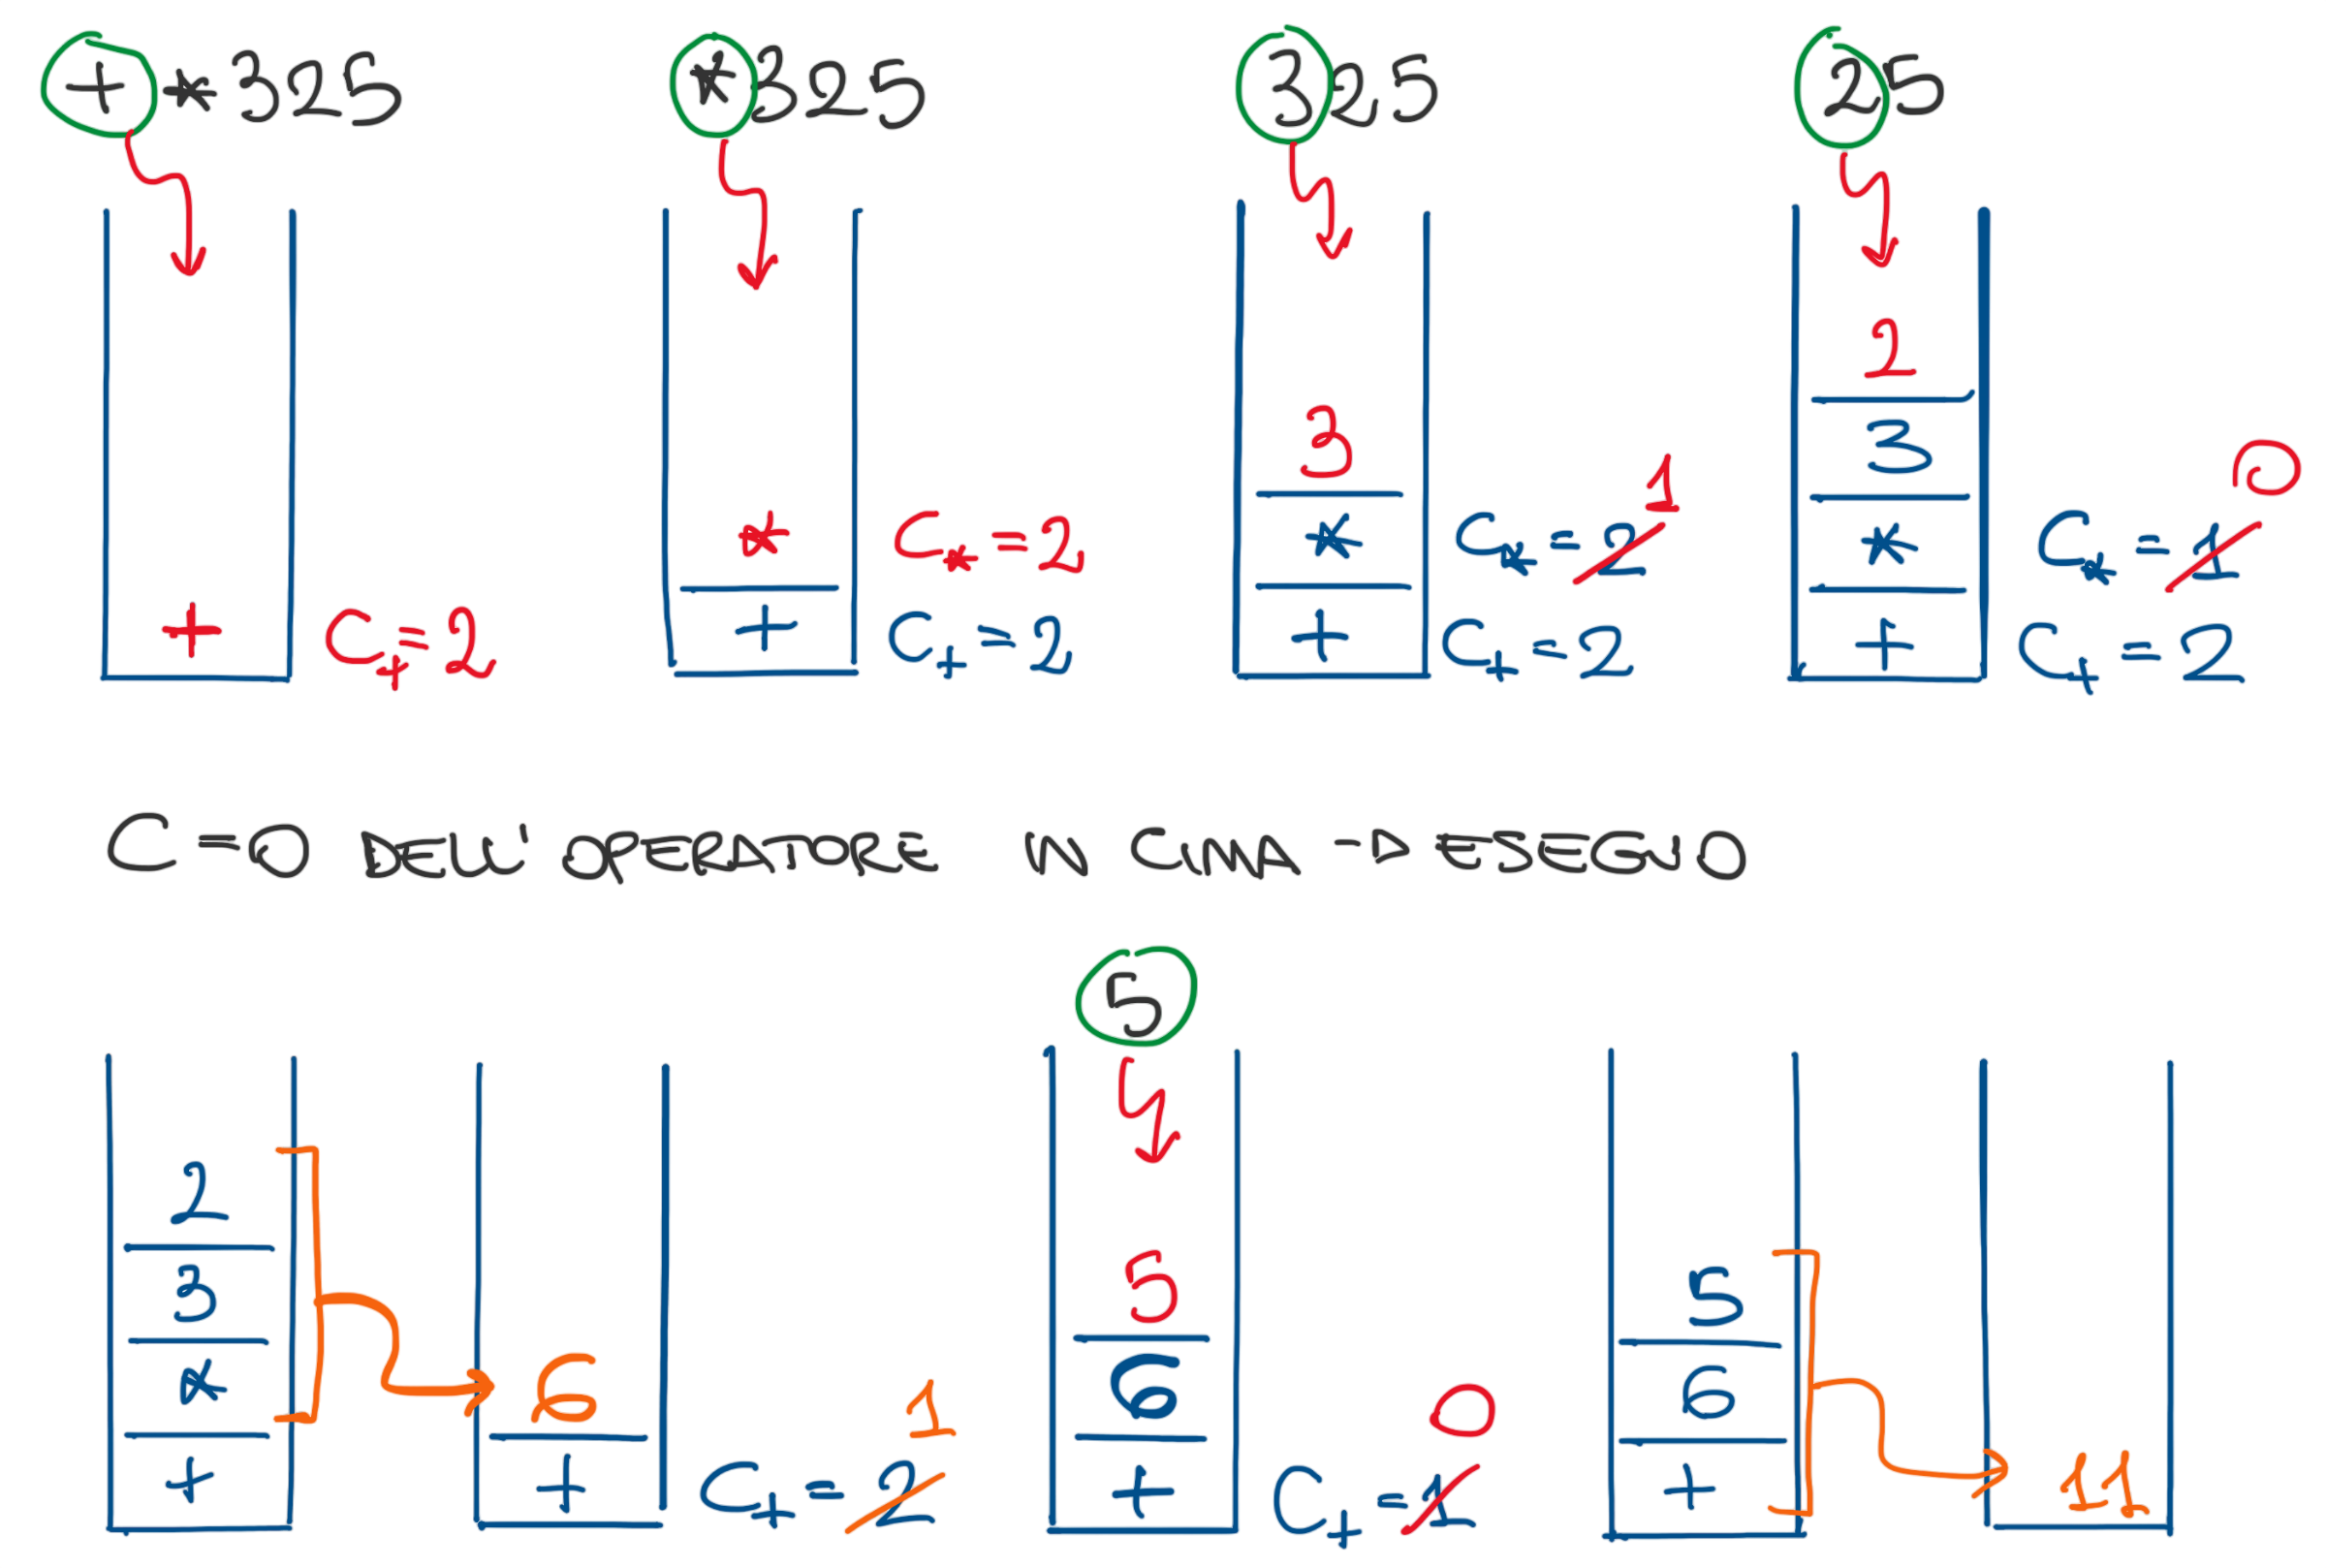
\includegraphics[width=\textwidth]{images/esempio-notazione-preFissa.png}
    \end{minipage}
}

\subsubsection{Notazione post-fissa}
La \textcolor{colore}{\textbf{notazione post-fissa}} è più semplice dell'in-fissa in quanto non necessita di regole di precedenza e associatività, e non necessita nemmeno di parentesi.

\vario{Algoritmo di valutazione}{
    \centering
    \begin{minipage}[c]{0.5\textwidth}
        \begin{enumerate}[itemsep=\smallskipamount]
            \item leggere il prossimo simbolo dell’espressione
            \begin{itemize}[label=$\triangleright$, itemsep=\smallskipamount]
                \item se il simbolo è un operatore (di varietà \texttt{n})
                \begin{itemize}[itemsep=\smallskipamount]
                    \item applicare l'operatore a \texttt{n} operandi immediatamente precedenti sulla pila
                    \item  memorizzare il risultato in \texttt{R}
                    \item eliminare operatore e operandi dalla pila
                    \item memorizzare il valore di \texttt{R} sulla pila
                \end{itemize}
                \item se il simbolo letto è un operando inserito nella pila
            \end{itemize}
            \item se ci sono ancora simboli nell'espressione da leggere tornare a 1 altrimenti terminare
        \end{enumerate}
    \end{minipage}
    \hfill
    \begin{minipage}[c]{0.45\textwidth}
        \centering
        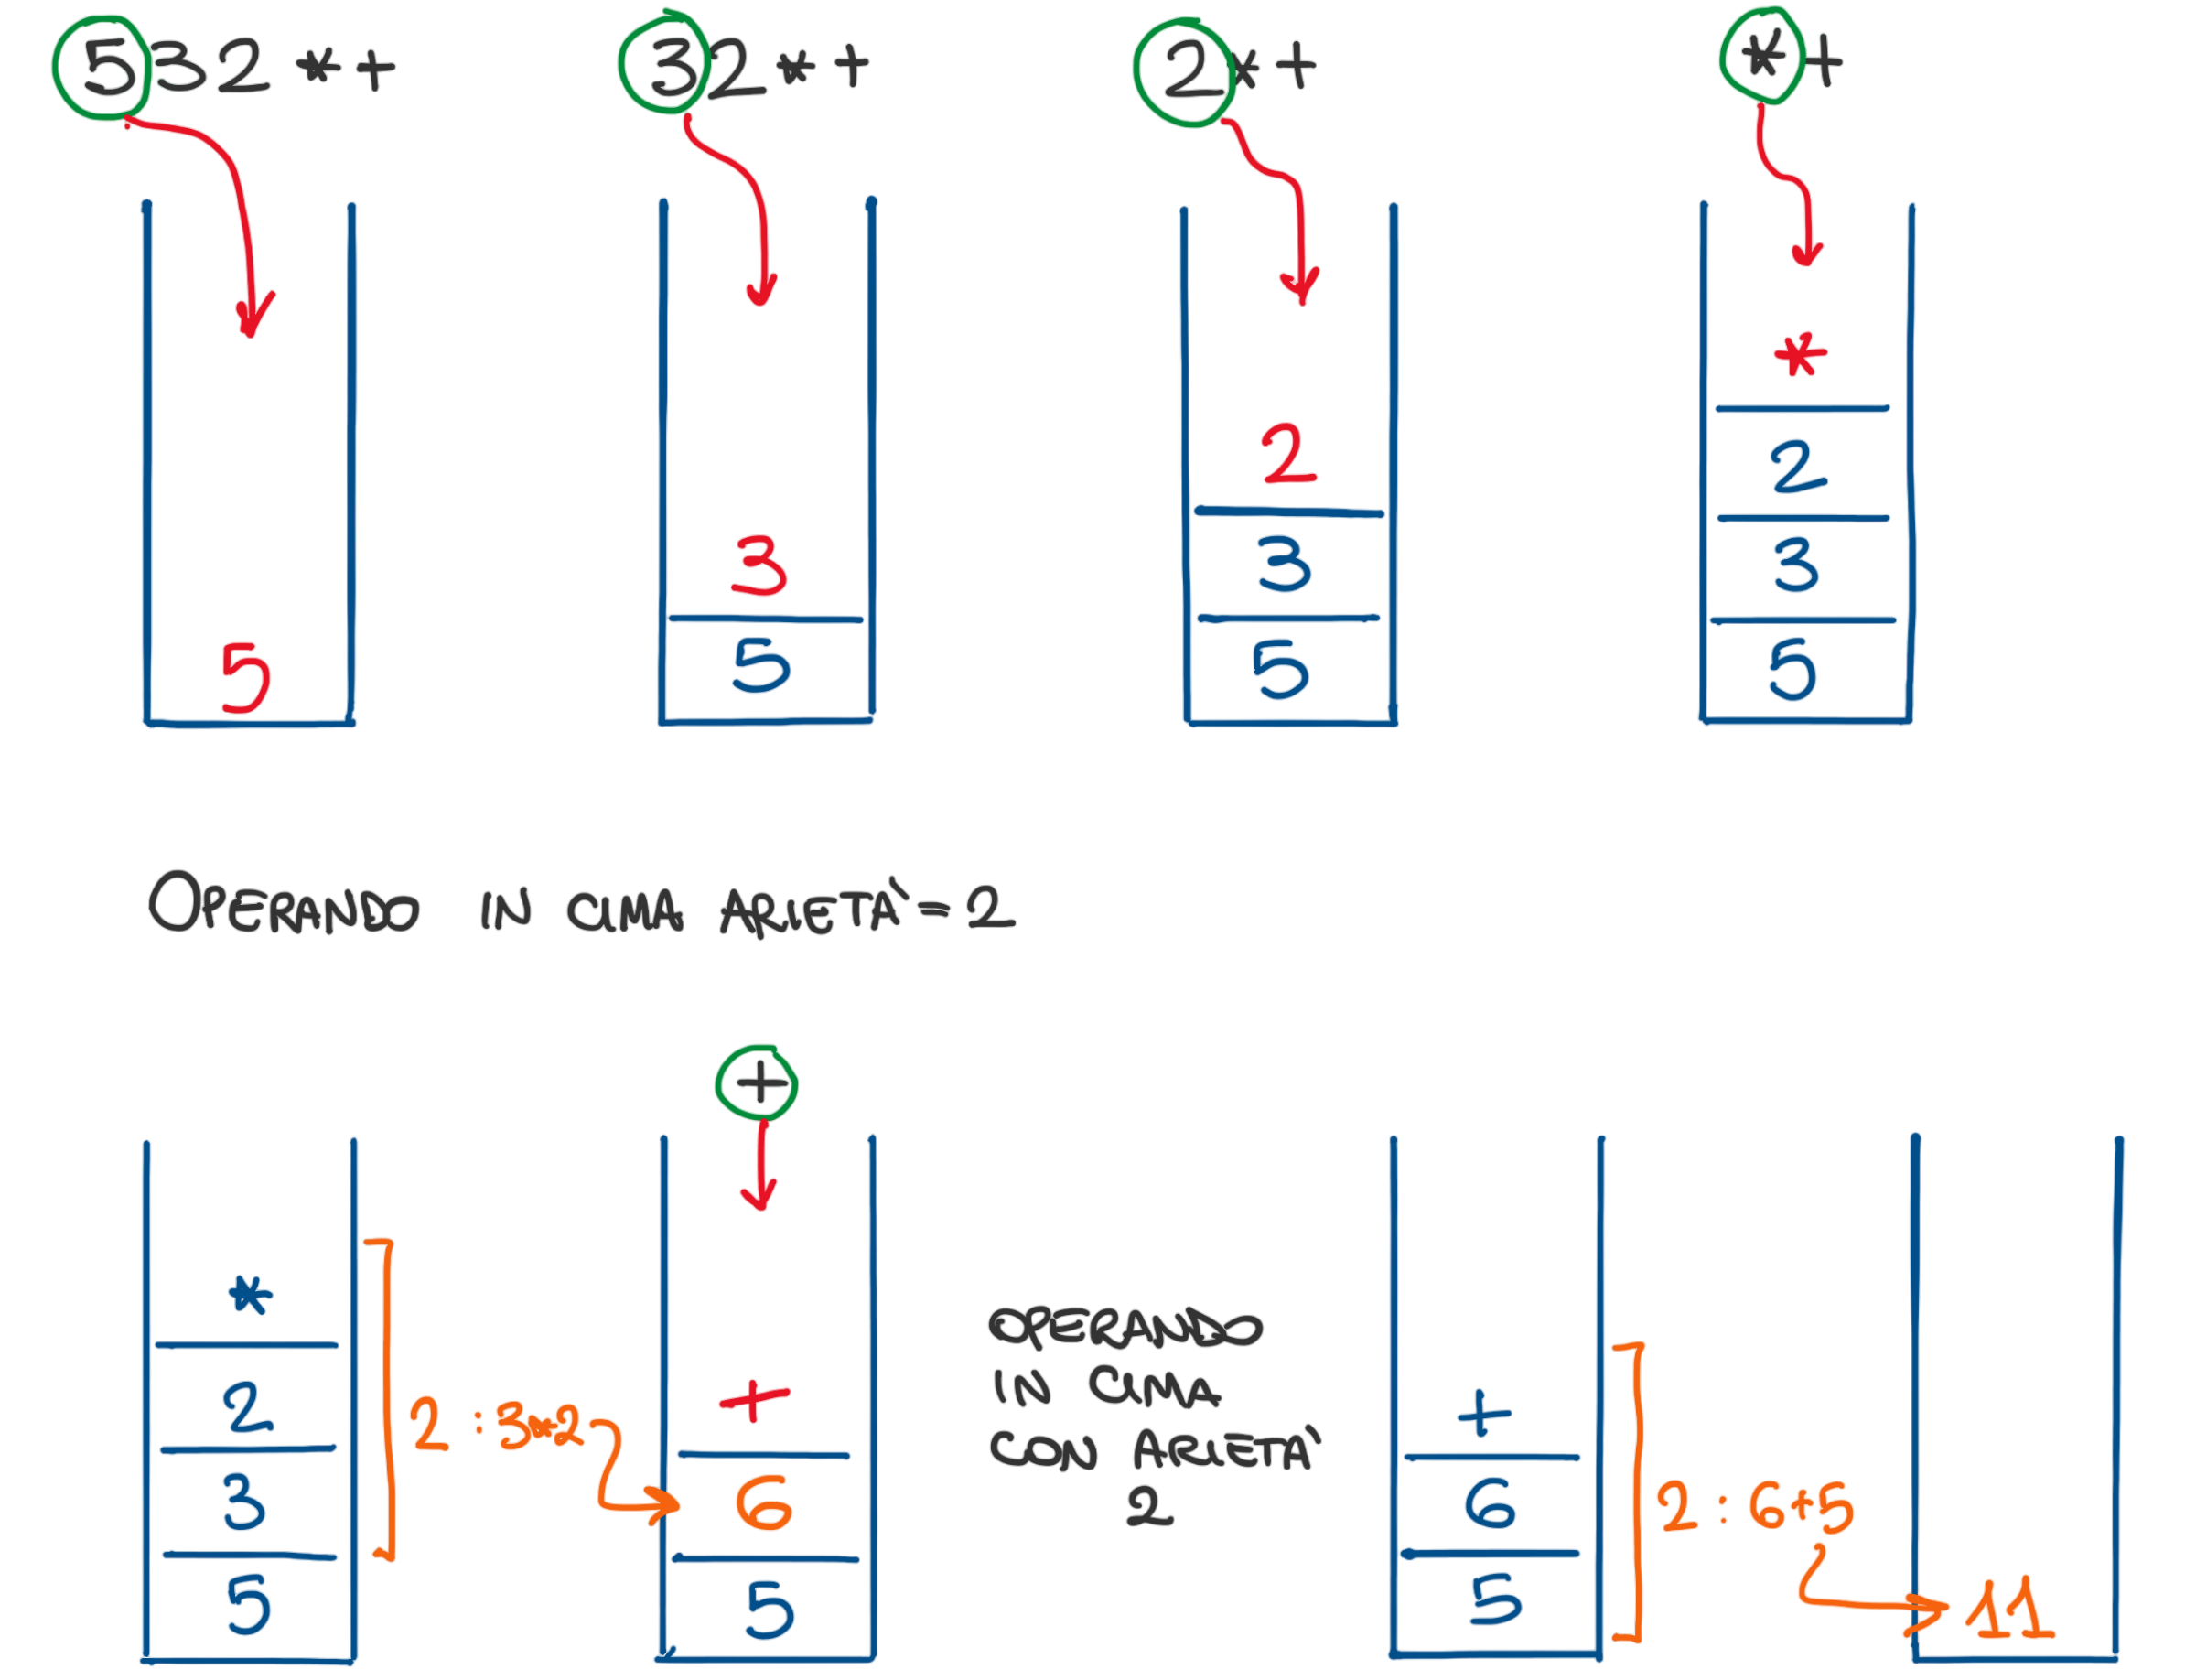
\includegraphics[width=\textwidth]{images/esempio-notazione-postFissa.png}
    \end{minipage}
}

\subsection{Regole di precedenza}
\begin{mydef}{regole di precedenza}
    Le \textbf{regole di precedenza} definiscono l'ordine in cui operatori "adiacenti" a diversi livelli di precedenza vengono valutati.
\end{mydef}

Tipici livelli di precedenza:
\begin{itemize}[label=$\triangleright$, itemsep=\smallskipamount]
    \item parentesi
    \item operatori unitari
    \item \texttt{**} (se esistono nel linguaggio)
    \item \texttt{*}, \texttt{/}
    \item \texttt{+}, \texttt{-}
\end{itemize}

\subsection{Regole di associatività}
\begin{mydef}{regole di associatività}
    Le \textbf{regole di associatività} stabiliscono l'ordine con cui operatori allo stesso livello di precedenza vengono valutati.
\end{mydef}

Tipiche regole di associatività:
\begin{itemize}[label=$\triangleright$, itemsep=\smallskipamount]
    \item da dx a sx
    \item operatori associano a dx (es. \text{FORTRAN})
    \item parentesi sovrasrivono le regole
\end{itemize}


\subsection{Valutazione delle espressioni}
La rappresentazione interna delle espressioni consiste in una rappresentazione ad albero.\\[0.2ex]
L'albero fornisce la struttura dell'espressione, ovvero elimina eventuali ambiguità legati a precedenze e associatività, ma non può dare informazioni rigurdanti l'ordine di valutazione dell'espressione in quanto ci sono vari aspetti che possono influire sil risultato:
\begin{itemize}[label=$\triangleright$, itemsep=\medskipamount]
    \item \textbf{operandi non definiti}: la presenza d operandi non definiti può far si che l'espressione risultante possa essere valutata solo con un preciso ordine di valutazione.
    
    \esempio{operandi non definiti}{
        Consideriamo questa espressione:
        \[
            \texttt{a == 0 ? b : b/a}
        \]
        
        Quando \texttt{a = 0} l'espressione da errore perchè \texttt{b/a} non è definita.

        E' vero, anche, che la valutazione di \texttt{b/a} avviene solo quando \texttt{a} è diverso da \texttt{0}.
    }

    A seconda del tipo di considerazioni possiamo avere:
    \begin{itemize}[label=$\Rightarrow$, itemsep=\smallskipamount]
        \item \textbf{valutazione eager}: vengono valutati sempre tutti gli operandi coinvolti
        \item \textbf{valutazione lazy}: gli operandi vengono valutati solo quando è necessario
    \end{itemize}
    \item \textbf{effetti collaterali} (side effect): sono effetti non propriamente legati all'oggetto che si sta manipolando (es. valutazione di un'espressione causa cambiamento della memoria o quando una funzione modifica i propri parametri)
    
    \esempio{effetti collaterali}{
        \[
            \begin{aligned}
                \texttt{a} &= 10;\\
                \texttt{b} &= \texttt{a} + \underbrace{\texttt{fun(a)}}_{\text{modifica valore di a per l'intero programma}}
            \end{aligned}
        \]
    }
    \item \textbf{aritmetica finita}: nelle macchine l'aritmetica è limitata dall'archiettura, quindi, i numeri non sono infiti ed esiste un massimo numero rappresentabile.
    
    Il problema di valutazione si ha in caso di espressioni che coinvolgono tale massimo numero.

    Tipicamente l'ordine di valutazione risolve il problema per prima cosa le variabili e le costanti poi valuta gli operandi seguendo la struttura data dalle parentesi dell'espressione.
\end{itemize}

\section{Sintassi}
La sintassi delle espressioni è la seguente:
\begin{bnfcode}{Sintassi delle espressioni}
    <Exp>
    E -> A | B
    A -> N | A op A
    B -> true | false | not B | B or B | A = A
\end{bnfcode}

dove:
\begin{itemize}[label=$\triangleright$, itemsep=\smallskipamount]
    \item \texttt{A}: espressioni aritmetiche
    \item \texttt{B}: espressioni booleane
    \item \texttt{N}: simboli che rappresentano numeri
    \item \texttt{op}: operatore numerico (\texttt{op} $\in \{+,-,*\}$)
\end{itemize}

\section{Semantica}
Definiamo il sistema di transizione che determina il processo di valutazione delle espressioni.\\[0.2ex]
Per definire un sistema di transizione di valutazione, abbiamo bisogno di definire:
\begin{itemize}[label=$\triangleright$, itemsep=\medskipamount]
    \item \textbf{configurazioni}: definite come $\Gamma = \epsilon$, ovvero le espressioni generate dalla grammatica.
    
    Il sottoinsieme $\mathrm{T} \subseteq \Gamma$ terminali sono $\mathrm{T} = \mathcal{N}$ (numerali della macchina su cui eseguiamo)
    \item \textbf{regole di transizione}: determina i passaggi di valutazione delle espressioni:
    \begin{itemize}[label=$\diamond$, itemsep=\medskipamount]
        \item espressioni aritmetiche: \texttt{op} $\in \{+,-,*\}$
        \item espressioni booleane: \texttt{bop} $\in \{or,+,-,*\}$
    \end{itemize}
\end{itemize}

\subsection{Regole di transizione: espressioni aritmetiche}
Le regole di transizione per le espressioni sono:
\begin{itemize}[label=$\circ$, itemsep=\medskipamount]
    \item \textbf{regola 1} (assioma): definisce \texttt{p} come la semantica del calcolo effettivo di un operatore
    \vario{regola $\mathcal{E}_1$ (assioma)}{
        \[
            \mathcal{E}_1: \underbrace{\mathrm{m} \textbf{ op } \mathrm{n} \to \mathrm{p}}_{\mathrm{m}, \ \mathrm{n}, \ \mathrm{p} \ \in \ \mathcal{N}} \quad \Leftrightarrow \quad \mathrm{m} \text{ op } \mathrm{n} = \mathrm{p}
        \]
    }
    \item \textbf{regola 2}: definsce la valutazione dell'espressione a sinistra per prima
    \vario{regola $\mathcal{E}_2$}{
        \[
            \mathcal{E}_2:\;
            \begin{prooftree}
                \hypo{\mathrm{e} \to \mathrm{e}'}
                \infer1{\mathrm{e} \texttt{ op } \mathrm{e}_0 \to \mathrm{e}' \texttt{ op } \mathrm{e}_0}
            \end{prooftree}
        \]
    }
    \item \textbf{regola 3}: definisce la valutazione dell'espressione a destra con un'espressione già valutata a sinistra
    \vario{regola $\mathcal{E}_3$}{
        \[
            \mathcal{E}_3:\;
            \begin{prooftree}
                \hypo{\mathrm{e} \to \mathrm{e}'}
                \infer1{\mathrm{m} \texttt{ op } \mathrm{e} \to \mathrm{m} \texttt{ op } \mathrm{e}'}
            \end{prooftree}
        \]
    }
\end{itemize}

\esempio{regole di transizione}{
    \begin{figure}[H]
        \centering
        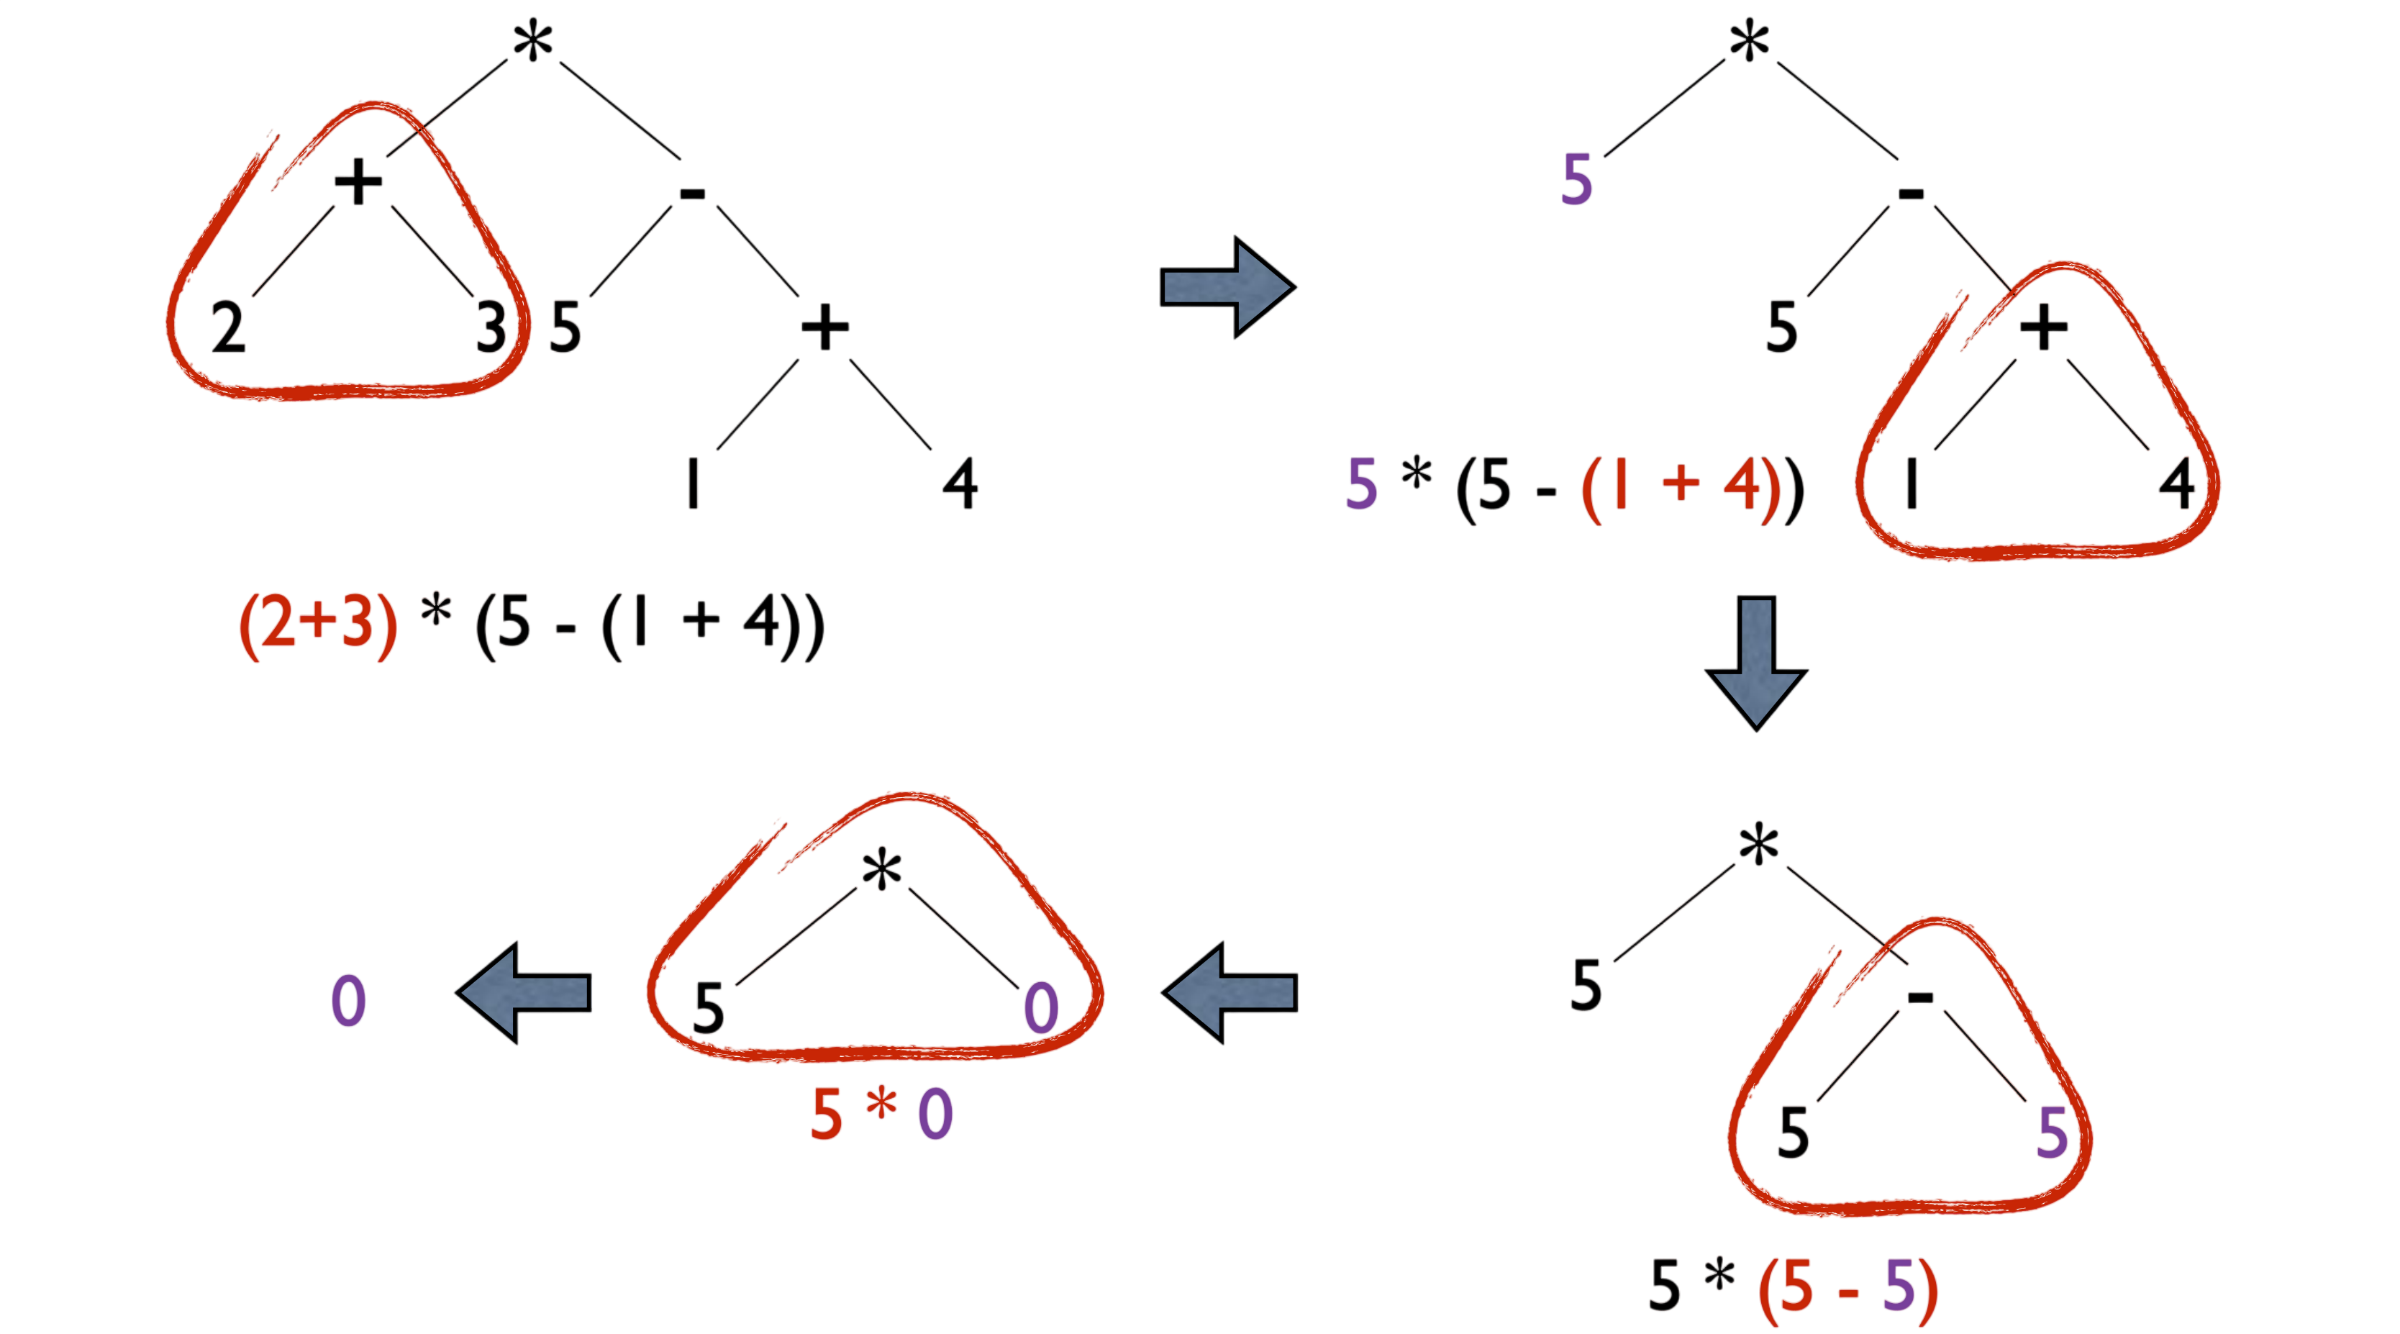
\includegraphics[width=0.8\textwidth]{images/regole-transioni-aritmetiche.png}
    \end{figure}
}

\subsubsection{Regole di transizione: espressioni booleane}
Le regole di transizione per le espressioni sono:
\begin{itemize}[label=$\circ$, itemsep=\medskipamount]
    \item \textbf{regola 4} (assioma):
    \vario{regola $\mathcal{E}_4$ (assioma)}{
        \[
            \mathcal{E}_4: \underbrace{\mathrm{k_1}}_{\in \ \mathcal{N} \ \cup \ \mathcal{B}} \texttt{ bop } \underbrace{\mathrm{k_2}}_{\in \ \mathcal{N} \ \cup \ \mathcal{B}} \to \underbrace{\mathrm{t}}_{\in \ \mathcal{B}} \Leftrightarrow \mathrm{k}_1 \texttt{ bop } \mathrm{k}_2 = \mathrm{t}
        \]
    }
    \item \textbf{regola 2'}:
    \vario{regola $\mathcal{E}_2'$}{
        \[
            \mathcal{E}_2':\;
            \begin{prooftree}
                \hypo{\mathrm{e} \to \mathrm{e'}}
                 \infer1{\mathrm{e} \texttt{ bop } \mathrm{e}_0 \to \mathrm{e}' \texttt{ bop } \mathrm{e}_0}
            \end{prooftree}
        \]
    }
    \item \textbf{regola 3'}:
    \vario{regola $\mathcal{E}_3'$}{
        \[
            \mathcal{E}_3':\;
            \begin{prooftree}
                \hypo{\mathrm{e} \to \mathrm{e'}}
                 \infer1{\mathrm{k} \texttt{ bop } \mathrm{e} \to \mathrm{k} \texttt{ bop } \mathrm{e}'}
            \end{prooftree}
        \]
    }
    \item \textbf{regola 5} (assioma):
    \vario{regola $\mathcal{E}_5$}{
        \[
            \mathcal{E}_{5}: \texttt{not } \underbrace{\mathrm{t}_0}_{\in \ \mathcal{B}} \rightarrow \underbrace{\mathrm{t}}_{\in \ \mathcal{B}} \Leftrightarrow \texttt{not } \mathrm{t}_0 = \mathrm{t}
        \]
    }
    \item \textbf{regola 6}:
    \vario{regola $\mathcal{E}_6$}{
        \[
            \mathcal{E}_6:\;
            \begin{prooftree}
                \hypo{\mathrm{e} \to \mathrm{e'}}
                 \infer1{\texttt{not } \mathrm{e} \to \texttt{not } \mathrm{e}'}
            \end{prooftree}
        \]
    }
\end{itemize}

Con queste regole di possono valutare ogni tipo di espressione.

\begin{mydef}{valutazione}
    Il processo di \textbf{valutazione} è una funzione:
    \[
        \mathrm{Eval}: \mathcal{E} \rightarrow \mathcal{N} \cup \mathcal{B} \mid \mathrm{Eval(e)} = \mathrm{k} \in \mathcal{N} \cup \mathcal{B} \Leftrightarrow \mathrm{e} \rightarrow *\mathrm{K}
    \]

    La valutazione di $\mathrm{e}$ è $\mathrm{k}$ se e solo se nel sistema di transizione con un certo numero di transizione possono transire da $\mathrm{e}$ a $\mathrm{k}$.
\end{mydef}

\begin{mydef}{equivalenza}
    La \textbf{relazione di equivalenza} è definita come:
    \[
        \equiv \ \subseteq \mathcal{E}_1 \times \mathcal{E}_2
    \]

    allora:
    \[
        \mathrm{e}_1 \equiv \mathrm{e}_2 \Leftrightarrow \mathrm{Eval(e_1)} = \mathrm{Eval(e_2)}
    \]
\end{mydef}